%-------------------------------------------------------------------------
\chapter{\babTiga}
%--------------------------------------------------------------------------
This chapter details the research methodology employed in this study. It includes descriptions of the dataset used, the overall system architecture, modifications made to the YOLO11 model, and the performance evaluation metrics applied to assess the effectiveness of the proposed approach.

\section{Dataset}
This research utilizes two primary datasets for training and evaluating the object detection models: the Dataset for Object Detection in Aerial Images (DOTA) and the Small Object Detection dAtaset (SODA). Both datasets are specifically designed for aerial imagery and present unique challenges for object detection tasks.

\subsection{DOTA Dataset}
The DOTA (Dataset for Object deTection in Aerial images) is a large-scale geospatial dataset widely used as a baseline for oriented object detection \cite{xia2019dotalargescaledatasetobject}. It is built from 2,806 high-resolution aerial images collected from different sensors and platforms, including Google Earth, to ensure a wide diversity of acquisition conditions. The images span from approximately $800 \times 800$ to $4,000 \times 4,000$ pixels, and together provide 188,282 annotated instances belonging to 15 common object categories such as plane, ship, storage tank, stadiums, harbor, bridge, large and small vehicles, helicopter, roundabout, and swimming pool. DOTA is split into training, validation, and test subsets with proportions of $1/2$, $1/6$, and $1/3$ respectively, which facilitates standard benchmarking protocols. Each instance is annotated with an Oriented Bounding Box (OBB) defined by four vertices $(x_i, y_i)$ arranged clockwise, which makes the dataset particularly suitable for aerial scenarios where objects appear at arbitrary rotations. The combination of extreme scale variation, dense object populations, and varying aspect ratios makes DOTA a challenging benchmark for evaluating object detection algorithms in aerial imagery. Figure \ref{fig:instances-dota} illustrates several instances from the DOTA dataset.

\begin{figure}
    \centering
    \includegraphics[width=1.0\textwidth]{pictures/instances-DOTA.jpg}
    \caption{Instances from the DOTA dataset.}\label{fig:instances-dota}
\end{figure}

\subsection{SODA Dataset}
The second dataset used in this research is the Small Object Detection dAtaset (SODA) benchmark \cite{Cheng_2023}, which contains two subsets tailored for driving (SODA-D) and aerial (SODA-A) scenarios. SODA-D spans 24,828 high-resolution street-level images with 278,433 instances labeled with Horizontal Bounding Boxes, while SODA-A focuses on aerial imagery and is the subset used in this research.

SODA-A comprises 2,513 aerial images harvested from Google Earth, each at an average resolution of $4761 \times 2777$ pixels to preserve the fine structure of tiny targets. The dataset contains 872,069 objects distributed over 9 classes, including Airplane, Helicopter, Small-vehicle, Large-vehicle, Ship, Container, Storage-tank, Swimming-pool, and Windmill. Data splits follow a 40\% / 25\% / 35\% ratio for training, validation, and testing, respectively. Similar to DOTA, annotations use Oriented Bounding Boxes (OBB) to capture rotated objects, but SODA-A explicitly targets the small-object challenge: objects with area under 1024 pixels are considered small, and the average instance size is only 14.75 pixels, with many instances qualifying as "Extremely Small" (area < 144 pixels). The dataset also exhibits extreme density, with some images containing over 11,000 instances, which compounds occlusion and background interference issues. These characteristics make SODA-A a demanding benchmark for evaluating detection performance on small, densely packed aerial targets. Figure \ref{fig:instances-soda} shows several instances from SODA-A.

\begin{figure}
    \centering
    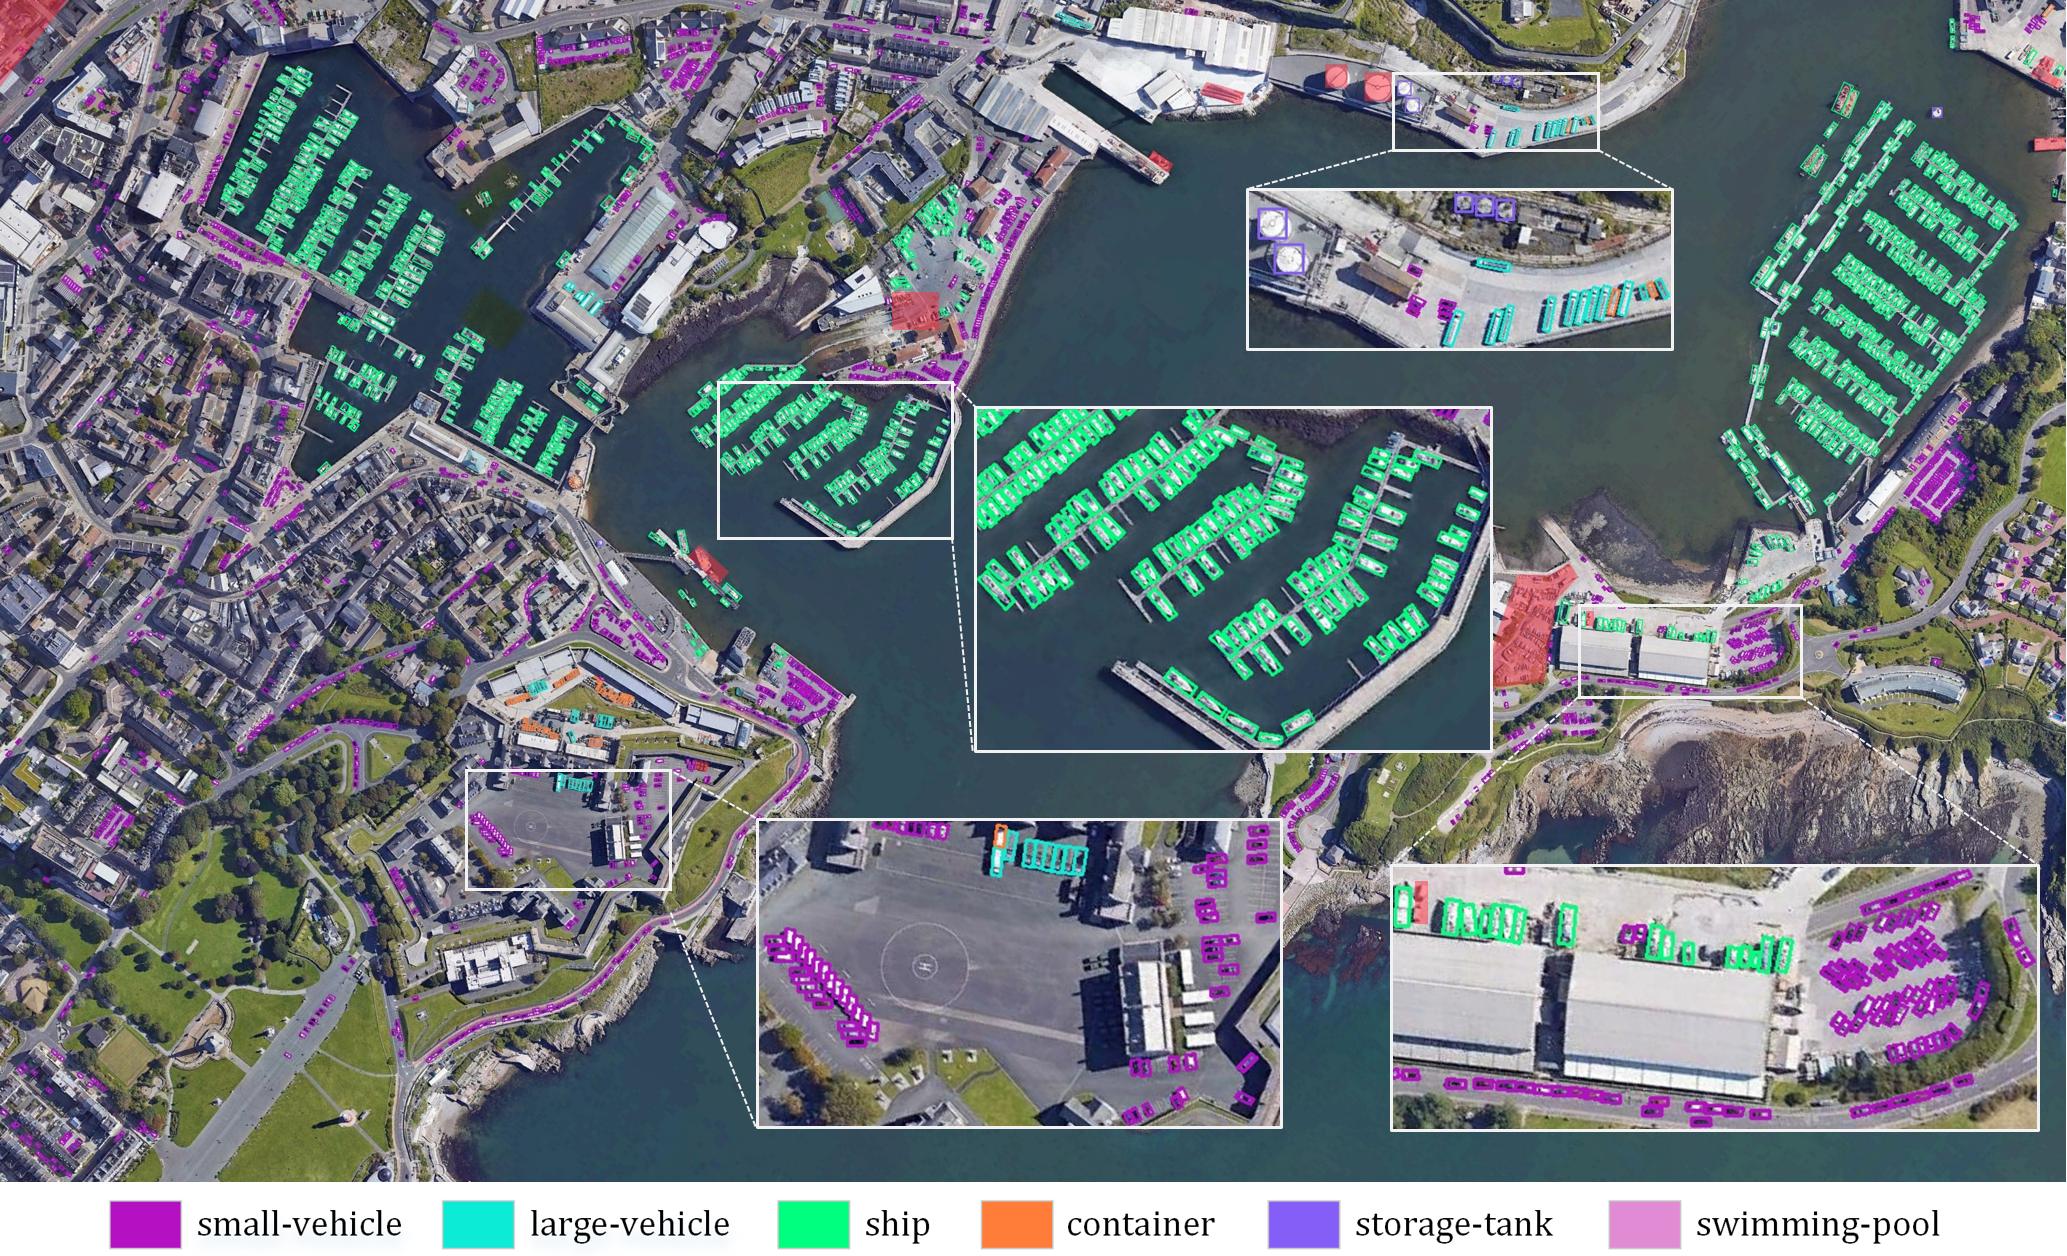
\includegraphics[width=1.0\textwidth]{pictures/SODA-A Vis.png}
    \caption{Instances from the SODA-A dataset.}
    \label{fig:instances-soda}
\end{figure}

The following Table \ref{tab:dataset-summary} summarizes the key features of both datasets used in this research.

\begin{table}[htbp]
    \centering
    \caption{Summary of DOTA and SODA-A Datasets.}
    \label{tab:dataset-summary}
    \resizebox{\textwidth}{!}{
    \begin{tabular}{|l|l|l|}
        \hline
        \multicolumn{1}{|c|}{\textbf{Feature}} & \multicolumn{1}{c|}{\textbf{DOTA}} & \multicolumn{1}{c|}{\textbf{SODA-A}} \\
        \hline
        Domain & General Aerial Detection & Small Object / Dense Aerial Detection \\
        Images & 2,806 & 2,513 \\
        Instances & 188,282 & 872,069 \\
        Categories & 15 & 9 \\
        Annotation Type & Oriented Bounding Box (OBB) & Oriented Bounding Box (OBB) \\
        Key Challenge & Scale Variation, Orientation & Extremely Small Objects, High Density \\
        \hline
    \end{tabular}
    }
\end{table}

\section{System Process Architecture}
Figure \ref{fig:system-process-architecture} illustrates the overall Experiment and Testing flow used in this research. The process begins with dataset preparation, where images and annotations from DOTA and SODA-A are standardized and converted into the annotation format required by the Ultralytics YOLO framework. The prepared dataset is then partitioned into training, validation, and testing subsets according to each dataset's predefined allocation ratios.

\begin{figure}
    \centering
    \includegraphics[width=0.7\textwidth]{pictures/Proposal Thesis - Experiment Diagram.png}
    \caption{System Process Architecture.}
    \label{fig:system-process-architecture}
\end{figure}

Next, the modified YOLO11 model is trained on the training set while monitoring validation performance to guide early stopping or further architecture tuning. When a trained checkpoint surpasses the established baseline, it is saved for later testing; otherwise, additional architectural modifications or hyperparameter adjustments are applied and the training loop repeats. The saved model is eventually loaded during the testing phase, where inference is performed on the unseen test set and the predicted boxes are compared to the ground-truth annotations to compute the evaluation metrics in this research. This system-wide process ensures that data collection, model development, and evaluation are tightly coordinated, which is essential for improving accuracy and efficiency in detecting aerial objects.

\section{Modified YOLO11 Architecture}
The proposed modifications to the YOLO11 architecture focus on enhancing its capability to detect oriented and small objects in aerial images. The key changes include integrating Deformable Convolutional Networks (DCN) into the backbone and neck of the model, as well as incorporating Deformable Attention mechanisms in the detection head. Figure \ref{fig:modified-yolo11-architecture} illustrates the overall architecture of the modified YOLO11 model.

\begin{figure}
    \centering
    \includegraphics[width=1.0\textwidth]{pictures/Architecture Proposal.png}
    \caption{(a) Baseline YOLO11 Architecture. (b) Modified YOLO11 Architecture with DCN and Deformable Attention.}
    \label{fig:modified-yolo11-architecture}
\end{figure}


\subsection{Deformable Convolution Networks (DCN)}
% rationale for DCN Integration


\subsection{Deformable Attention}
% rationale for Deformable Attention Integration

\section{Performance Evaluation Metrics} 
In this research, the performance of the modified YOLO11 model is evaluated using standard object detection metrics, primarily focusing on Mean Average Precision (mAP) at different Intersection over Union (IoU) thresholds. Others metrics such as Precision, Recall, and F1-Score are also computed to provide a comprehensive assessment of the model's detection capabilities, especially in handling oriented and small objects in aerial imagery. To quantify computational cost, we also track the number of model parameters (Params) and Floating Point Operations per Second (FLOPS), ensuring that accuracy improvements remain practical for real-world deployment.

\subsection{Precision}
Precision measures the proportion of correctly predicted positive instances (true positives) out of all instances predicted as positive (true positives + false positives). It reflects the model's ability to avoid false alarms.

\begin{equation}
    \mathrm{Precision} = \frac{TP}{TP + FP}
\end{equation}

where \( TP \) is the number of true positives and \( FP \) is the number of false positives.

\subsection{Recall}
Recall measures the proportion of correctly predicted positive instances (true positives) out of all actual positive instances (true positives + false negatives). It indicates the model's ability to detect all relevant objects.

\begin{equation}
    \mathrm{Recall} = \frac{TP}{TP + FN}
\end{equation}

where \( TP \) is the number of true positives and \( FN \) is the number of false negatives.

\subsection{F1-Score}
The F1-Score is the harmonic mean of Precision and Recall, providing a single metric that balances both aspects of model performance. It is particularly useful when the class distribution is imbalanced.

\begin{equation}
    \mathrm{F1\text{-}Score} = 2 \times \frac{\mathrm{Precision} \times \mathrm{Recall}}{\mathrm{Precision} + \mathrm{Recall}}
\end{equation}

\subsection{Mean Average Precision (mAP)}
Mean Average Precision (mAP) is the primary metric used to evaluate the object detection performance of the model. It is calculated by averaging the Average Precision (AP) across all object classes. AP is derived from the Precision-Recall curve for each class, which plots precision against recall at various confidence thresholds. The mAP is computed at different IoU thresholds (e.g., mAP@0.5, mAP@0.50-95) to assess how well the model detects objects with varying degrees of overlap with ground truth boxes. 

\begin{equation}
    \mathrm{mAP} = \frac{1}{N} \sum_{i=1}^{N} AP_i
    \label{eq:map}
\end{equation}

where \( N \) is the number of classes and \( AP_i \) is the Average Precision for class \( i \).

\subsection{Number of Parameters (Params)}
The number of parameters (Params) in the model quantifies its complexity and size. It is calculated by summing all learnable weights and biases across all layers of the neural network. A lower number of parameters generally indicates a more efficient model, which is beneficial for deployment in resource-constrained environments.

\begin{equation}
    \mathrm{Params} = \sum_{i=1}^{L} (W_i + B_i)
\end{equation}

where \( L \) is the number of layers, \( W_i \) is the number of weights in layer \( i \), and \( B_i \) is the number of biases in layer \( i \).

\subsection{Floating Point Operations per Second (FLOPS)}
FLOPS measures the computational efficiency of the model by counting the number of floating-point operations required to process a single input image. It provides insight into the model's speed and resource requirements, which are critical for real-time applications.

\begin{equation}
    \mathrm{FLOPS} = \sum_{i=1}^{L} F_i
\end{equation}

where \( L \) is the number of layers and \( F_i \) is the number of floating-point operations in layer \( i \).